%TODO:
% Apply defintiions
% Short introduction to Architecture qualities
As software engineers our focus is on creating a software architecture based on the architectural requirements. Software architecture allows us to reasons and take qualified decision. It is essential that we early in the project    \cite{un}

\section{Quality Attributes}
We will follow the definition on software architecture from \cite{Bass}. 
%**************************************Definition Software architecture
\begin{defi}[\textbf{Software architecture}]
The software architecture of a system is the set of \textbf{structures} needed to reason about the system, which comprise software \textbf{elements}, \textbf{relations} among them, and the \textbf{properties} of both. 
\end{defi}
%**************************************Definition Software architecture End

\noindent
Our approach towards implementing a software architecture is based on Quality attribute (QA) and Quality attribute scenario (QAS). A quality attribute (QA) according to \cite{Bass} is as follows.

%**************************************Definition Quality attribute
\begin{defi}[\textbf{Quality attribute}]
..A quality attribute is a measurable or testable property of a system that is used to indicate how well the satisfies the needs of its stakeholders..  
\end{defi}
%**************************************Definition Quality attribute End


% TODO:
% Introduction to QA
% List relevant quality attributes
% Why these attributes?
% Relate to generel mobile application challenges and tactics
\noindent
From \cite{Bass} we have seven quality attributes here among modifiability, availability and performance. Furthermore \cite{Kjaergaard:2015:AQT:2737182.2737196} has added energy efficiency and and ressources adaptability.  



\section{Quality Attribute Scenarios}
% TODO:
% Formal definition of QAS
% Use template from Bass
\noindent
A core observation is that a QA should be measurable or testable quality. The key point is when working with QA we use them in a given context/scenario and therefor we informally call these as QAS.\\



\begin{figure}[H]
\centering
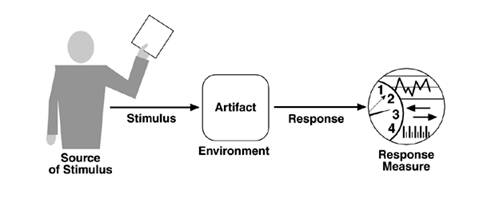
\includegraphics[scale=0.8]{QualityAttributeScenario.jpg}

\caption{The parts of a quality attribute scenario}
\label{fig:Quality_Attribute_Scenario}
\end{figure}





\noindent
One of the core aspects of the definition of software architecture, is that software architecture is a set of structures, which we can use to reason about the system. To assist and visualize these structures, elements, relations and properties we use Module-, Component \& Connector (C\&C)- and Allocation viewpoints \cite{3+1}. 

\begin{enumerate}
    \item Module viewpoint is concerned with how functionality of the system maps to static development units. The focus will be on elements such as classes and interfaces and relationships such as associations, generalizations, realizations and dependencies.
    \item Component \& Connector viewpoint is concerned with the runtime mapping of functionality to components of the architecture. Components are the executing things that perform a function. Connectors are the communication channels between components. The purpose is to focus on the flow of data and responsibilities such as a network call or method call etc.
    \item Allocation viewpoint is concerned with how software entities are mapped to environmental entities. Here the focus are on the physical stuff such as computer or a network. We specify the environment in order to make the software running. 
\end{enumerate}

\noindent
These viewpoint originates from $3+1$ article \cite{3+1}, where the $+1$ is the architectural requirements. These architectural requirements can be formulated through QAS.


\begin{table}[H]
\begin{center}
\begin{tabular}{|p{0.3cm}|p{2.5cm}|p{8cm}|}
  \hline
  \multicolumn{2}{|p{3cm}|}{\bfseries Scenario(s):} & \#  5: A developer should be able to make a change to the random number generator code under runtime and the change are made and tested within 3 hours. \\
  \hline
  \multicolumn{2}{|p{3cm}|}{\bfseries Relevant Quality Attributes:} & Modifiability\\
  \hline
  \multirow{6}{*}{\begin{sideways}{\bfseries Scenario Parts}\end{sideways}}
  & {\bfseries Source:} & Developer \\
  \cline{2-3}
  & {\bfseries Stimulus:} & Needs to replace the random generator \\
  \cline{2-3}
  & {\bfseries Artifact} &  Code \\
  \cline{2-3}
  & {\bfseries Environment:} &  Design time \\
  \cline{2-3}
  & {\bfseries Response:} &  Replacement made and Unit tested\\
  \cline{2-3}
  & {\bfseries Response Measure:} & In three hours\\
  \hline
\end{tabular}
\caption{Modifiability QAS}
\end{center}
\end{table}


\section{Tactics}
% TODO:
% For each QA find tactics
% Examples
%   - Performance: Limit sampling rate
%       - Possible solution: Our hierarachy divide and 
%         conquer
%   - Modifiability: Encapsulation/coupling/cohesion
%       - Possible solution: Interfaces, multiple APIs 
%         and storage
%   - Availability: Redundancy (caching layer)
%       - Possible solution: local caching

\noindent
We will discuss different tactics on software architecture for achieving the business goal for the electronic voting application. A tactic according to \cite{Bass} is defined as.

%**************************************Definition Tactic
\begin{defi}[\textbf{Tactic}]
Tactic is a design decision that influences the achievement of a quality attribute response. 
\end{defi}
%**************************************Definition Tactic End